\documentclass{article}
\usepackage{listings}
\usepackage{fullpage}
\usepackage{graphicx}
\begin{document}
\section{Maximum clique decision problem}
Given a graph $G$ and an integer $k$, find a subgraph of $G$ of size $k$ isomorphic to $C_k$. In this case we are only interested in getting a yes/no answer.
\section{Constraint programming}
A constraint modelling language MiniZinc was used to model the problem. Each model has variables and constraints. Each variable has a domain of possible values.

For each variable, a constraint solver keeps either its current value or a subset of its domain that it still deems possible. It then repeats the following two steps:
\begin{enumerate}
\item Inference. For each constraint and for each possible value in each (remaining) domain, check if that value is still possible.
\item Search. Choose a free variable according to a heuristic and choose one of its possible values according to some rule. Set the variable equal to that value and recurse.
\end{enumerate}
\section{Initial model}
\begin{lstlisting}
include "globals.mzn";

int: n; % number of vertices
int: k; % size of the clique we're looking for
array[1..n,1..n] of 0..1: adjacent; % adjacency matrix
array[1..n] of var 0..1: clique; % whether a vertex is part of the clique

constraint sum(clique) == k;
constraint forall(i, j in 1..n where i != j)(
    clique[i] == 1 /\ clique[j] == 1 -> adjacent[i,j] == 1);
solve satisfy;
\end{lstlisting}
A script was implemented to generate graphs with a set number of vertices and a probability of having an edge between every two vertices.
\begin{figure}
  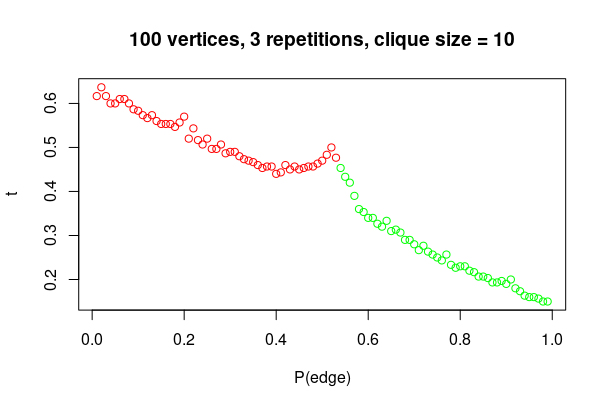
\includegraphics[scale=0.5]{max_clique.png}
  \label{fig:initial_max_clique}
\end{figure}
\ref{fig:initial_max_clique} shows how the running time (in seconds) changed by changing the edge probability for a graph with 100 vertices looking for a clique of size 10, averaged out over 3 different graphs. Each data point is marked green if a clique of required size was found most of the time (2 out of 3 runs) and red otherwise.

Surprisingly, this model takes the longest time for graphs with almost no edges. To explain that, consider two things: 1) how guesses are ordered during the search, and 2) when inference can actually reduce domain sizes.

Usually, variables are ordered by domain size, but in this case all domains are of size 2, so the actual ordering is essentially random. The algorithm has no way of knowing which values it should try first, so the default ordering is increasing, which means that we are guessing which vertices are not in the clique until all the remaining vertices have to be in the clique. Hence, switching the order could reduce the average height of the search tree. The variable ordering could also be improved by ordering vertices by their degree in either increasing or decreasing order.

The first constraint is easily checked and marks the remaining vertices as part of the clique once that is the only way to satisfy the constraint. According to the optimized FlatZinc file, the second constraint is actually transformed to its contrapositive and for every non-edge, it checks that one of the incident vertices is not in the clique. For sparse graphs, that is $O(|V|^2)$ of work.
\section{Improvements}
To produce a more optimized FlatZinc file, the number of constraints was reduced in half by considering each pair of vertices only once (enforcing $j<i$).
\end{document}
